\documentclass[12pt]{book}

% Packages for better formatting
\usepackage{geometry} % Page layout
\usepackage{titlesec} % Formatting headings
\usepackage{fancyhdr} % Header/Footer
\usepackage{hyperref} % Hyperlinks
\usepackage{graphicx} % For images
\usepackage{amsmath} % For math
\usepackage{amssymb} % For math symbols
\usepackage{enumitem} % Custom lists
\usepackage[most]{tcolorbox}
\usepackage{epstopdf} % For converting EPS to PDF

% Page layout
\geometry{a4paper, margin=1in}

% Header and footer
\pagestyle{fancy}
\fancyhf{}
\fancyhead[L]{Extra HAM!}
\fancyhead[R]{}
\fancyfoot[C]{\thepage}

% Title formatting
\titleformat{\chapter}[hang]{\huge\bfseries}{Chapter \thechapter}{1em}{}
\titleformat{\section}[hang]{\Large\bfseries}{\thesection}{0.5em}{}

% Hyperlink setup
\hypersetup{
    colorlinks=true,
    linkcolor=blue,
    filecolor=magenta,
    urlcolor=cyan,
    pdftitle={Extra HAM!},
    pdfauthor={Charles Perng},
    bookmarks=true,
    pdfpagemode=FullScreen,
}

\begin{document}

% Title page
\begin{titlepage}
    \centering
    {\Huge\bfseries Extra HAM! \\
    \vspace{0.5cm}
    A Test Preparation Guide \\
    \vspace{1cm}
    \large By Charles Perng}
    
    \vspace{4cm}
    \includegraphics[width=\textwidth]{extra-ham.png} % Specify width
    % or use \includegraphics[width=\textwidth]{extra-ham.pdf} if converted
    
    \vfill
    {\large \today}
\end{titlepage}

% Table of Contents
\tableofcontents
\newpage

% Preface
\chapter*{Preface}
This book, \textit{Extra HAM!}, is designed to help you prepare for the HAM radio licensing exams. With a mix of theoretical explanations and practical exercises, you will develop the skills and confidence to ace your test. Let’s dive in!

\newpage

% Chapter 1
% ************************************************************************
% CHAPTER 1: Sublement E1 - Commission Rules
% ************************************************************************
\chapter{E1: Commission Rules}

% ------------------------------------------------------------------------
% SECTION E1A: Frequency Privileges and Band Restrictions
% ------------------------------------------------------------------------
\section{E1A: Frequency Privileges and Band Restrictions}

\subsection*{Understanding the Basics}
  \textcolor{myblue}{\textbf{Frequency privileges}} in amateur radio refers to the specific ranges of radio frequencies that licensed amateur operators are allowed to use. These bands are not random; they are allocated by international and national regulatory bodies. Each band has different propagation characteristics that make them suitable for different types of communication.
  \par
  \textcolor{myblue}{\textbf{Power restrictions}} dictate how much output power your transmitter can use. These are also band-specific. Some bands, like 630- and 2200-meter bands, have lower power limits due to their unique propagation and interference potential.
  \par
  It is very important that all users operate within allocated bands and power restrictions for that band.
  
\mybox{mygreen}{
  \textbf{Fun Fact}: The 630-meter and 2200-meter bands are relatively new additions to the US amateur radio allocation, offering hams a taste of "low-band" propagation!  These bands have unique challenges and opportunities for experimentation, allowing for long-distance communications through ground-wave and sky-wave propagation. They also require notifications and special operating procedures.
  }
  
\subsection*{Key Concepts for the Questions}
\begin{itemize}
    \item \textbf{HF (High Frequency) Bands:} These range from approximately 3 to 30 MHz and offer various long-distance communications opportunities.
    \item \textbf{Band Edges:}  The upper and lower limits of a specific frequency band.
    \item \textbf{USB/LSB (Upper Sideband/Lower Sideband):} Two common modes of transmission in the HF bands. They are different types of Amplitude Modulation where carrier is suppressed and only one side band is transmitted. In general Upper Sideband is used for bands with a central frequency of above 10 MHz and LSB is used otherwise.
    \item \textbf{Phone Mode:} The modulation for carrying voice. It often uses single side band.
    \item \textbf{Data Mode}: A wide variety of modulation used for digital data transmissions.
    \item \textbf{Carrier Frequency:} The base frequency at which a radio signal is transmitted.
    \item \textbf{Bandwidth:} The range of frequencies that a signal occupies.
\end{itemize}

\subsection*{Practice Questions}
\begin{enumerate}
    \item Why is it not legal to transmit a 3 kHz bandwidth USB signal with a carrier frequency of 14.348 MHz?
    \begin{enumerate}
        \item USB is not used on 20-meter phone
        \item  The lower 1 kHz of the signal is outside the 20-meter band
        \item  14.348 MHz is outside the 20-meter band
        \item  \textbf {The upper 1 kHz of the signal is outside the 20-meter band}
    \end{enumerate}
    \textcolor{myred}{Explanation:}
    The 20-meter amateur band is roughly from 14.000 to 14.350 MHz. When transmitting in USB mode, the carrier frequency is at the bottom of transmitted signal. For 3 KHz signal, the top of the signal is at 14.351 MHz which is out of the permitted band, therefore is not legal.
        
    \item When using a transceiver that displays the carrier frequency of phone signals, which of the following displayed frequencies represents the lowest frequency at which a properly adjusted LSB emission will be totally within the band?
    \begin{enumerate}
        \item The exact lower band edge
        \item  300 Hz above the lower band edge
        \item  1 kHz above the lower band edge
        \item \textbf {3 kHz above the lower band edge}
    \end{enumerate}
    \textcolor{myred}{Explanation:}
    When transmitting in LSB mode, the carrier frequency is at the top of the transmitted signal. For a 3 kHz bandwidth signal, the lower end will be 3 kHz below the displayed frequency. For the signal to be in the band, the lowest end of the signal needs to be at the band edge. Thus the displayed carrier frequency should be 3 kHz above the band edge.
    
        \item What is the highest legal carrier frequency on the 20-meter band for transmitting a 2.8 kHz wide USB data signal?
    \begin{enumerate}
        \item 14.0708 MHz
         \item  14.1002 MHz
         \item \textbf {14.1472 MHz}
        \item  14.3490 MHz
    \end{enumerate}
    \textcolor{myred}{Explanation:}
    The highest end of 20m band is 14.350 MHz. Because we are using USB mode, our carrier frequency will be on the lower end of the signal, thus, the carrier can go up to 14.350 MHz - 2.8 KHz = 14.3472 MHz. The data portion of the 20 meter band ends at 14.150 MHz. The highest legal carrier frequency is then 14.150 MHz-0.0028 MHz = 14.1472 MHz.

    
        \item May an Extra class operator answer the CQ of a station on 3.601 MHz LSB phone?
    \begin{enumerate}
        \item Yes, the entire signal will be inside the SSB allocation for Extra class operators
        \item  Yes, the displayed frequency is within the 75-meter phone band segment
        \item \textbf {No, the sideband components will extend beyond the edge of the phone band segment}
         \item  No, US stations are not permitted to use phone emissions below 3.610 MHz
        \end{enumerate}
         \textcolor{myred}{Explanation:}
          Extra class operators have voice allocation above 3.600 MHz. The lowest edge of the phone segment is 3.600 MHz. If we are using LSB and transmitting at 3.601 MHz, the lower side band goes below 3.600 MHz. Thus, the signal will extend beyond the band edge and become illegal.
          
      \item Who must be in physical control of the station apparatus of an amateur station aboard any vessel or craft that is documented or registered in the United States?
\begin{enumerate}
   \item Only a person with an FCC Marine Radio license grant
\item  Only a person named in an amateur station license grant
\item \textbf {Any person holding an FCC issued amateur license or who is authorized for alien reciprocal operation}
\item  Any person named in an amateur station license grant or a person holding an unrestricted Radiotelephone Operator Permit
\end{enumerate}
\textcolor{myred}{Explanation:}
Any licensed amateur operator can operate the station on a vessel or aircraft. There is no need for any special endorsement.
 
    \item What is the required transmit frequency of a CW signal for channelized 60 meter operation?
    \begin{enumerate}
        \item At the lowest frequency of the channel
        \item \textbf {At the center frequency of the channel}
        \item  At the highest frequency of the channel
        \item  On any frequency where the signal's sidebands are within the channel
    \end{enumerate}
     \textcolor{myred}{Explanation:}
    The 60-meter band has specific channels and each channel has center frequencies for CW operations.

    \item What is the maximum power permitted on the 2200-meter band?
    \begin{enumerate}
        \item 50 watts PEP (peak envelope power)
        \item  100 watts PEP (peak envelope power)
         \item \textbf {1 watt EIRP (equivalent isotropic radiated power)}
        \item  5 watts EIRP (equivalent isotropic radiated power)
    \end{enumerate}
    \textcolor{myred}{Explanation:}
     The 2200 meter band is among the newest allocations and has special restrictions, including the use of EIRP for power limitation, that is different from the traditional PEP method.

      \item If a station in a message forwarding system inadvertently forwards a message that is in violation of FCC rules, who is primarily accountable for the rules violation?
    \begin{enumerate}
        \item The control operator of the packet bulletin board station
        \item \textbf {The control operator of the originating station}
        \item  The control operators of all the stations in the system
        \item  The control operators of all the stations in the system not authenticating the source from which they accept communications
    \end{enumerate}
      \textcolor{myred}{Explanation:}
     The control operator of the originating station is responsible for ensuring the contents of any transmission is within FCC regulations, regardless of how it is forwarded.
       
      \item Except in some parts of Alaska, what is the maximum power permitted on the 630-meter band?
        \begin{enumerate}
       \item 50 watts PEP (peak envelope power)
      \item  100 watts PEP (peak envelope power)
       \item  1 watt EIRP (equivalent isotropic radiated power)
        \item \textbf {5 watts EIRP (equivalent isotropic radiated power)}
    \end{enumerate}
        \textcolor{myred}{Explanation:}
         The 630 meter band has special restrictions, including the use of EIRP for power limitation, that is different from the traditional PEP method.
         
      \item If an amateur station is installed aboard a ship or aircraft, what condition must be met before the station is operated?
        \begin{enumerate}
        \item \textbf {Its operation must be approved by the master of the ship or the pilot in command of the aircraft}
       \item  The amateur station operator must agree not to transmit when the main radio of the ship or aircraft is in use
       \item  The amateur station must have a power supply that is completely independent of the main ship or aircraft power supply
        \item  The amateur station must operate only in specific segments of the amateur service HF and VHF bands
     \end{enumerate}
        \textcolor{myred}{Explanation:}
    If operating on a ship or aircraft, the master or pilot must give approval before operating the station.
      
    \item What licensing is required when operating an amateur station aboard a US-registered vessel in international waters?
      \begin{enumerate}
     \item Any amateur license with an FCC Marine or Aircraft endorsement
    \item \textbf {Any FCC-issued amateur license}
       \item  Only General class or higher amateur licenses
     \item  An unrestricted Radiotelephone Operator Permit
      \end{enumerate}
     \textcolor{myred}{Explanation:}
      Any FCC issued amateur radio license will grant operator access on a US registered vessel in international water. There is no requirement for marine or aircraft endorsement.
\end{enumerate}


% ------------------------------------------------------------------------
% SECTION E1B: Station Restrictions and Special Operations
% ------------------------------------------------------------------------
\section{E1B: Station Restrictions and Special Operations}

\subsection*{Understanding the Basics}
  \textcolor{myblue}{\textbf{Station restrictions}} cover various aspects of your amateur radio operation. These can include limits on where you can set up a station, how high your antennas can be, what kind of emissions are permitted, and more. These restrictions are in place to minimize interference with other radio services and to ensure that your station operation doesn't negatively affect public safety.
  \par
  \textcolor{myblue}{\textbf{Spurious emissions}} are any emissions outside the intended bandwidth of your signal. This is important because these unwanted signals can interfere with other radio services. These are controlled by FCC regulations.
  \par
  \textcolor{myblue}{\textbf{RACES (Radio Amateur Civil Emergency Service)}} is a special operating program for amateur radio during emergencies. It often allows for use of restricted frequencies during emergencies. 
   \mybox{mygreen}{
      \textbf{Fun Fact}: Did you know that many of the rules and regulations that we follow today were developed based on a combination of historical precedence and new technological development? Regulations often balance the need for access to frequencies with the goal of minimizing interference, especially among essential services.
      }

\subsection*{Key Concepts for the Questions}
\begin{itemize}
    \item \textbf{Spurious Emissions:} Unwanted signals outside the necessary bandwidth of a transmission.
    \item \textbf{Necessary Bandwidth:} The minimum bandwidth required to transmit the information in a signal.
    \item \textbf{FCC Monitoring Facility:} A location where the Federal Communications Commission monitors radio activity.
    \item \textbf{RACES:} Radio Amateur Civil Emergency Service; a service providing emergency communications.
    \item \textbf{Public Use Airport:} An airport used by commercial and private aircraft.
    \item \textbf{PRB-1:}  A federal document that establishes guidelines for zoning regulations affecting amateur radio antennas.
    \item \textbf{Notam (Notice to Air Missions):}  A notice filed with FAA when construction of tall structures can become hazards to the air crafts
\end{itemize}

\subsection*{Practice Questions}
\begin{enumerate}
    \item Which of the following constitutes a spurious emission?
    \begin{enumerate}
        \item An amateur station transmission made without the proper call sign identification
        \item  A signal transmitted to prevent its detection by any station other than the intended recipient
        \item  Any transmitted signal that unintentionally interferes with another licensed radio station and whose levels exceed 40 dB below the fundamental power level
        \item \textbf {An emission outside the signal's necessary bandwidth that can be reduced or eliminated without affecting the information transmitted}
    \end{enumerate}
    \textcolor{myred}{Explanation:}
    A spurious emission is any emission from a transmitter that is outside its designed bandwidth, which can be eliminated without sacrificing the content of transmission.

     \item Which of the following is an acceptable bandwidth for digital voice or slow-scan TV transmissions made on the HF amateur bands?
    \begin{enumerate}
        \item \textbf {3 kHz}
        \item  10 kHz
        \item  15 kHz
        \item  20 kHz
    \end{enumerate}
       \textcolor{myred}{Explanation:}
   While there are some exception, 3 kHz is the most common limit for digital voice and slow-scan TV signals on the HF bands. This is to make sure those signal does not interfere with the other signals in the band.

       \item Within what distance must an amateur station protect an FCC monitoring facility from harmful interference?
       \begin{enumerate}
         \item \textbf {1 mile}
         \item  3 miles
         \item  10 miles
        \item  30 miles
        \end{enumerate}
        \textcolor{myred}{Explanation:}
    The FCC mandates that amateur stations must protect FCC monitoring facilities within 1 mile from harmful interference.
    
       \item What must the control operator of a repeater operating in the 70-centimeter band do if a radiolocation system experiences interference from that repeater?
       \begin{enumerate}
        \item Reduce the repeater antenna HAAT (Height Above Average Terrain)
         \item  File an FAA NOTAM (Notice to Air Missions) with the repeater system's ERP, call sign, and six-character grid locator
       \item \textbf {Cease operation or make changes to the repeater that mitigate the interference}
        \item  All these choices are correct
        \end{enumerate}
          \textcolor{myred}{Explanation:}
      The control operator must make changes to the repeater or cease the operation to mitigate interference with radiolocation.
        
         \item What is the National Radio Quiet Zone?
       \begin{enumerate}
          \item An area surrounding the FCC monitoring station in Laurel, Maryland
      \item  An area in New Mexico surrounding the White Sands Test Area
    \item \textbf {An area surrounding the National Radio Astronomy Observatory}
       \item  An area in Florida surrounding Cape Canaveral
        \end{enumerate}
          \textcolor{myred}{Explanation:}
       The National Radio Quiet Zone surrounds the National Radio Astronomy Observatory in West Virginia and limits certain radio transmissions.
       
        \item Which of the following additional rules apply if you are erecting an amateur station antenna structure at a site at or near a public use airport?
        \begin{enumerate}
        \item \textbf {You may have to notify the Federal Aviation Administration and register it with the FCC as required by Part 17 of the FCC rules}
       \item  You may have to enter the height above ground in meters, and the latitude and longitude in degrees, minutes, and seconds on the FAA website
         \item  You must file an Environmental Impact Statement with the EPA before construction begins
    \item  You must obtain a construction permit from the airport zoning authority per Part 119 of the FAA regulations
      \end{enumerate}
    \textcolor{myred}{Explanation:}
     Antenna construction near an airport must follow part 17 of the FCC rules and may require notification of FAA.
     
    \item To what type of regulations does PRB-1 apply?
      \begin{enumerate}
          \item Homeowners associations
       \item  FAA tower height limits
      \item \textbf {State and local zoning}
       \item  Use of wireless devices in vehicles
        \end{enumerate}
     \textcolor{myred}{Explanation:}
     PRB-1 is for zoning regulations and establish guidance for state and local zoning rules when regarding the construction of radio antennas.
    
       \item What limitations may the FCC place on an amateur station if its signal causes interference to domestic broadcast reception, assuming that the receivers involved are of good engineering design?
      \begin{enumerate}
          \item The amateur station must cease operation
      \item  The amateur station must cease operation on all frequencies below 30 MHz
         \item  The amateur station must cease operation on all frequencies above 30 MHz
      \item \textbf {The amateur station must avoid transmitting during certain hours on frequencies that cause the interference}
      \end{enumerate}
    \textcolor{myred}{Explanation:}
    If a station signal is causing interference with broadcasting reception, FCC can request avoidance of transmission in those frequencies when the interference is happening.
       
      \item Which amateur stations may be operated under RACES rules?
        \begin{enumerate}
          \item Only those club stations licensed to Amateur Extra class operators
       \item  Any FCC-licensed amateur station except a Technician class
     \item \textbf {Any FCC-licensed amateur station certified by the responsible civil defense organization for the area served}
     \item  Only stations meeting the FCC Part 97 technical standards for operation during an emergency
    \end{enumerate}
    \textcolor{myred}{Explanation:}
    Any FCC-licensed amateur radio can operate under RACES rules if certified by the local civil defense organization.
     
    \item What frequencies are authorized to an amateur station operating under RACES rules?
    \begin{enumerate}
      \item \textbf {All amateur service frequencies authorized to the control operator}
    \item  Specific segments in the amateur service MF, HF, VHF, and UHF bands
    \item  Specific local government channels
        \item  All these choices are correct
    \end{enumerate}
     \textcolor{myred}{Explanation:}
     A RACES operation may use all amateur radio bands and modes authorized to the control operator.
    
    \item What does PRB-1 require of state and local regulations affecting amateur radio antenna size and structures?
    \begin{enumerate}
        \item No limitations may be placed on antenna size or placement
        \item \textbf {Reasonable accommodations of amateur radio must be made}
        \item  Such structures must be permitted when use for emergency communications can be demonstrated
        \item  Such structures must be permitted if certified by a registered professional engineer
        \end{enumerate}
     \textcolor{myred}{Explanation:}
     PRB-1 dictates that zoning rules should be applied with reasonable accommodations for amateur radio.
\end{enumerate}

% ------------------------------------------------------------------------
% SECTION E1C: Automatic and Remote Control
% ------------------------------------------------------------------------
\section{E1C: Automatic and Remote Control}
\subsection*{Understanding the Basics}
  \textcolor{myblue}{\textbf{Automatic control}} refers to the operation of a ham radio station without the direct, active participation of a control operator. This can involve computer programs, timers, or other automation.
  \par
  \textcolor{myblue}{\textbf{Remote control}} involves operation of a station over a distance, typically using radio links or the internet. While remote operation provides great flexibility, it also requires careful attention to regulations.
  \par
  \textcolor{myblue}{\textbf{Band-specific regulations}} can be very different. It is essential to be familiar with these requirements.
   \par
  \textcolor{myblue}{\textbf{Spurious emission standards}} are very important to prevent interference to other communication services.
  \par
  \textcolor{myblue}{\textbf{HF modulation index limit}} is important for the voice operation, as explained in E8B.
  \par

  \subsection*{Deep Dive}
  
\subsubsection*{Modulation Index}

The \textbf{modulation index} is a measure of the extent of modulation in an amplitude modulation (AM) system. It is defined as the ratio of the amplitude of the modulating signal to the amplitude of the carrier signal. Mathematically, it is expressed as:

\begin{equation}
    m = \frac{A_m}{A_c}
\end{equation}

where:
\begin{itemize}
    \item $m$ is the modulation index,
    \item $A_m$ is the amplitude of the modulating signal,
    \item $A_c$ is the amplitude of the carrier signal.
\end{itemize}

The modulation index determines the characteristics of the AM signal:
\begin{itemize}
    \item \textbf{Under-Modulation:} $m < 1$, where the modulating signal is weaker than the carrier signal.
    \item \textbf{Critical Modulation:} $m = 1$, where the amplitude of the modulating signal equals the amplitude of the carrier signal.
    \item \textbf{Over-Modulation:} $m > 1$, where the modulating signal is stronger than the carrier signal, leading to distortion.
\end{itemize}

\subsubsection*{Illustration of Modulated Waveforms}
Below are the waveform illustrations for normal modulation (critical modulation) and over-modulation:



\begin{figure}[h!]
    \centering
    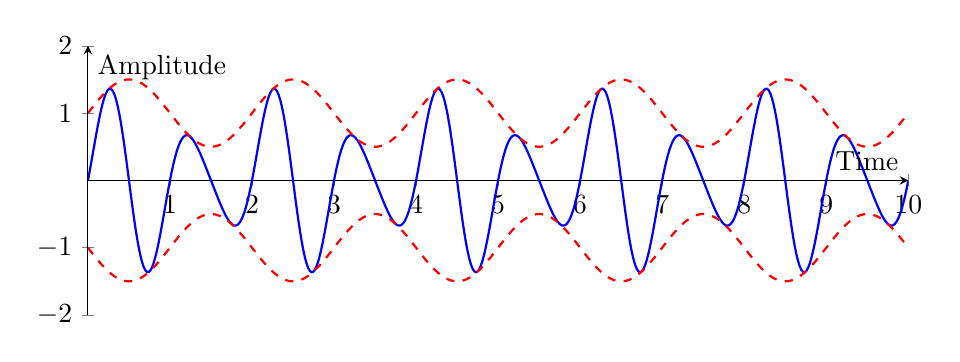
\begin{tikzpicture}
        \begin{axis}[
            width=12cm, height=5cm,
            xlabel={Time}, ylabel={Amplitude},
            axis lines=middle,
            xmin=0, xmax=10,
            ymin=-2, ymax=2,
            samples=500,
        ]
        % Normal modulation
        \addplot [blue, thick, domain=0:10] { (1 + 0.5*sin(deg(2*pi*x/2)))*sin(deg(2*pi*x)) };
        \addplot [red, thick, dashed, domain=0:10] { 1 + 0.5*sin(deg(2*pi*x/2)) };
        \addplot [red, thick, dashed, domain=0:10] { -1 - 0.5*sin(deg(2*pi*x/2)) };
        \end{axis}
    \end{tikzpicture}
    \caption{Normal Modulation ($m = 1$)}

    \vspace{1cm}

    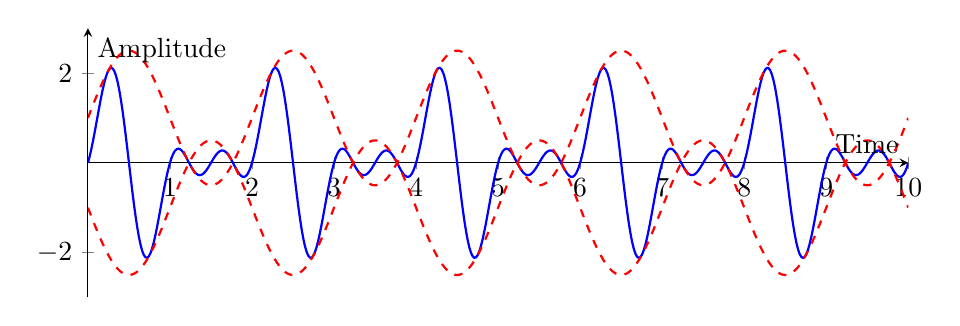
\begin{tikzpicture}
        \begin{axis}[
            width=12cm, height=5cm,
            xlabel={Time}, ylabel={Amplitude},
            axis lines=middle,
            xmin=0, xmax=10,
            ymin=-3, ymax=3,
            samples=500,
        ]
        % Over-modulation
        \addplot [blue, thick, domain=0:10] { (1 + 1.5*sin(deg(2*pi*x/2)))*sin(deg(2*pi*x)) };
        \addplot [red, thick, dashed, domain=0:10] { 1 + 1.5*sin(deg(2*pi*x/2)) };
        \addplot [red, thick, dashed, domain=0:10] { -1 - 1.5*sin(deg(2*pi*x/2)) };
        \end{axis}
    \end{tikzpicture}
    \caption{Over-Modulation ($m > 1$)}
%\caption{Illustrations of AM waveforms: Normal Modulation and Over-Modulation}
\end{figure}

  
\mybox{mygreen}{
    \textbf{Fun Fact}:  Modern technology has enabled hams to operate their station remotely from halfway around the world using Internet and radio links, adding new dimensions to amateur radio. But the fundamental rules related to transmission and interference still apply.
    }


\subsection*{Key Concepts for the Questions}
\begin{itemize}
    \item \textbf{Data emission:}  Digital signals used for transferring information.
    \item \textbf{Foreign Communications:} Transmissions sent to or received from amateur stations in other countries.
    \item \textbf{IARP:} International Amateur Radio Permit; enables operations in countries in Americas.
    \item \textbf{CEPT:} European Conference of Postal and Telecommunications administrations. Enables operations in most European countries.
    \item \textbf{Third Party Communications:} Passing messages on behalf of other people, not the operator.
    \item \textbf{Utilities Technology Council (UTC):} An organization that facilitates notification before operation on specific bands.
    \item \textbf{Angle modulation:} A type of modulation where the information is encoded in the phase or frequency.
    \item \textbf{Spurious emission:} Unwanted radio signals transmitted outside the desired bandwidth.
\end{itemize}

\subsection*{Practice Questions}
\begin{enumerate}
    \item What is the maximum bandwidth for a data emission on 60 meters?
        \begin{enumerate}
       \item 60 Hz
        \item  170 Hz
      \item  1.5 kHz
        \item \textbf {2.8 kHz}
    \end{enumerate}
     \textcolor{myred}{Explanation:}
     The FCC specifies the maximum bandwidth of 2.8 kHz for digital modes on the 60-meter band.
        
        \item Which of the following apply to communications transmitted to amateur stations in foreign countries?
    \begin{enumerate}
        \item Third party traffic must be limited to that intended for the exclusive use of government and non-Government Organization (NGOs) involved in emergency relief activities
        \item  All transmissions must be in English
        \item \textbf {Communications must be limited to those incidental to the purpose of the amateur service and remarks of a personal nature}
        \item  All these choices are correct
    \end{enumerate}
     \textcolor{myred}{Explanation:}
    Transmissions to stations in foreign countries must be non-commercial, non-political and limited to personal topics.
        
        \item How long must an operator wait after filing a notification with the Utilities Technology Council (UTC) before operating on the 2200-meter or 630-meter band?
        \begin{enumerate}
          \item Operators must not operate until approval is received
       \item \textbf {Operators may operate after 30 days, providing they have not been told that their station is within 1 kilometer of PLC systems using those frequencies}
      \item  Operators may not operate until a test signal has been transmitted in coordination with the local power company
    \item  Operations may commence immediately, and may continue unless interference is reported by the UTC
       \end{enumerate}
       \textcolor{myred}{Explanation:}
      Once the operator files a notification to UTC for operations in 2200m and 630m band, operation can commence after 30 days.
        
        \item What is an IARP?
       \begin{enumerate}
        \item \textbf {A permit that allows US amateurs to operate in certain countries of the Americas}
         \item  The internal amateur radio practices policy of the FCC
        \item  An indication of increased antenna reflected power
       \item  A forecast of intermittent aurora radio propagation
        \end{enumerate}
        \textcolor{myred}{Explanation:}
      IARP or International Amateur Radio Permit allows operations in select countries in Americas.

    \item Under what situation may a station transmit third party communications while being automatically controlled?
        \begin{enumerate}
        \item Never
          \item \textbf {Only when transmitting RTTY or data emissions}
         \item  Only when transmitting SSB or CW
        \item  On any mode approved by the National Telecommunication and Information Administration
     \end{enumerate}
       \textcolor{myred}{Explanation:}
        Third party communications can only be transmitted in data mode and under automatic control.

    \item Which of the following is required in order to operate in accordance with CEPT rules in foreign countries where permitted?
       \begin{enumerate}
         \item You must identify in the official language of the country in which you are operating
    \item  The US embassy must approve of your operation
    \item \textbf {You must have a copy of FCC Public Notice DA 16-1048}
        \item  You must append "/CEPT" to your call sign
    \end{enumerate}
        \textcolor{myred}{Explanation:}
     FCC public notice DA 16-1048 lists conditions of operations under CEPT.

     \item What notifications must be given before transmitting on the 630- or 2200-meter bands?
   \begin{enumerate}
         \item A special endorsement must be requested from the FCC
       \item  An environmental impact statement must be filed with the Department of the Interior
    \item  Operators must inform the FAA of their intent to operate, giving their call sign and distance to the nearest runway
      \item \textbf {Operators must inform the Utilities Technology Council (UTC) of their call sign and coordinates of the station}
    \end{enumerate}
        \textcolor{myred}{Explanation:}
         To start operations in 630m or 2200m band the operators must inform UTC about their call sign and coordinates.
      
        \item What is the maximum permissible duration of a remotely controlled station's transmissions if its control link malfunctions?
         \begin{enumerate}
         \item 30 seconds
        \item \textbf {3 minutes}
      \item  5 minutes
        \item  10 minutes
        \end{enumerate}
           \textcolor{myred}{Explanation:}
         If remote control malfunctions, the station can only transmit for maximum 3 minutes.
        
        \item What is the highest modulation index permitted at the highest modulation frequency for angle modulation below 29.0 MHz?
       \begin{enumerate}
        \item 0.5
        \item \textbf {1.0}
       \item  2.0
      \item  3.0
     \end{enumerate}
       \textcolor{myred}{Explanation:}
    The modulation index must be less than 1.0 for any angle modulation below 29 MHz.
        
       \item What is the maximum mean power level for a spurious emission below 30 MHz with respect to the fundamental emission?
        \begin{enumerate}
     \item \textbf {- 43 dB}
        \item  - 53 dB
       \item  - 63 dB
        \item  - 73 dB
    \end{enumerate}
   \textcolor{myred}{Explanation:}
    The power of a spurious emission below 30 MHz must be at least 43 dB less than fundamental power.
       
     \item Which of the following operating arrangements allows an FCC-licensed US citizen to operate in many European countries, and amateurs from many European countries to operate in the US?
      \begin{enumerate}
      \item \textbf {CEPT}
        \item  IARP
      \item  ITU reciprocal license
     \item  All these choices are correct
      \end{enumerate}
      \textcolor{myred}{Explanation:}
       CEPT allows reciprocal operations in many European countries as well as the US.

        \item In what portion of the 630-meter band are phone emissions permitted?
         \begin{enumerate}
          \item None
          \item  Only the top 3 kHz
           \item  Only the bottom 3 kHz
       \item \textbf {The entire band}
       \end{enumerate}
        \textcolor{myred}{Explanation:}
     Phone operation is permitted throughout the 630 meter band.
\end{enumerate}


% ------------------------------------------------------------------------
% SECTION E1D: Amateur Space and Earth Stations
% ------------------------------------------------------------------------
\section{E1D: Amateur Space and Earth Stations}
\subsection*{Understanding the Basics}
   \textcolor{myblue}{\textbf{Amateur space and earth stations}} are radio facilities for communicating through satellites and balloons that are more than 50 km above the Earth's surface. They have special rules regarding telemetry, telecommand, and identification.
\par
   \textcolor{myblue}{\textbf{Telemetry}} refers to the transmission of data or measurements to a ground station.
   \textcolor{myblue}{\textbf{Telecommand}} signals are used to remotely control the station. These communications follow specific rules in order to reduce interference with the other services and operations.
   \textcolor{myblue}{\textbf{One-way communications}} are usually prohibited but is allowed for beacons and space stations.

\mybox{mygreen}{
  \textbf{Fun Fact}: Some of the most exciting amateur radio activities occur through satellite communications. The International Space Station (ISS) often has amateur radio gear onboard that can be used to talk with astronauts! There are also a whole collection of small amateur satellites that you can contact.
  }


\subsection*{Key Concepts for the Questions}
\begin{itemize}
    \item \textbf{Telemetry:} The one way transmission of measurements.
        \item \textbf{Telecommand:} The signals that control a remote system.
    \item \textbf{Space Telecommand Station:} The earth station that sends telecommand signals to space.
    \item \textbf{One-way transmission:} Transmission from a station with no response from the receiving station.
     \item \textbf{Earth Station:} An amateur station that communicates with the space station.
      \item \textbf{HF/VHF/UHF Bands:} High frequency, very high frequency, and ultra high frequency amateur bands.
      \item \textbf{AMASAT:} Radio Amateur Satellite Corporation

\end{itemize}

\subsection*{Practice Questions}
\begin{enumerate}
  \item What is the definition of telemetry?
    \begin{enumerate}
        \item \textbf {One-way transmission of measurements at a distance from the measuring instrument}
        \item  Two-way transmissions in excess of 1000 feet
       \item  Two-way transmissions of data
        \item  One-way transmission that initiates, modifies, or terminates the functions of a device at a distance
    \end{enumerate}
    \textcolor{myred}{Explanation:}
    Telemetry is the transmission of data from a remote location for measurement. It is a one way communication.

    \item Which of the following may transmit encrypted messages?
     \begin{enumerate}
        \item Telecommand signals to terrestrial repeaters
        \item \textbf {Telecommand signals from a space telecommand station}
        \item  Auxiliary relay links carrying repeater audio
        \item  Mesh network backbone nodes
    \end{enumerate}
      \textcolor{myred}{Explanation:}
    Only space telecommand station may transmit encrypted messages.
    
    \item What is a space telecommand station?
    \begin{enumerate}
      \item An amateur station located on the surface of the Earth for communication with other Earth stations by means of Earth satellites
        \item \textbf {An amateur station that transmits communications to initiate, modify, or terminate functions of a space station}
     \item  An amateur station located in a satellite or a balloon more than 50 kilometers above the surface of the Earth
        \item  An amateur station that receives telemetry from a satellite or balloon more than 50 kilometers above the surface of the Earth
    \end{enumerate}
       \textcolor{myred}{Explanation:}
    A space telecommand station is a station on earth that sends telecommand to satellites and other space stations.

    \item Which of the following is required in the identification transmissions from a balloon-borne telemetry station?
       \begin{enumerate}
          \item \textbf {Call sign}
        \item  The output power of the balloon transmitter
        \item  The station's six-character Maidenhead grid locator
        \item  All these choices are correct
    \end{enumerate}
         \textcolor{myred}{Explanation:}
    A ballon-born telemetry station is required to identify by callsign at the beginning of the transmission.
    
        \item What must be posted at the location of a station being operated by telecommand on or within 50 kilometers of the Earth's surface?
      \begin{enumerate}
        \item A photocopy of the station license
        \item  A label with the name, address, and telephone number of the station licensee
    \item  A label with the name, address, and telephone number of the control operator
      \item \textbf {All these choices are correct}
    \end{enumerate}
          \textcolor{myred}{Explanation:}
     At a telecommand station, the station license, licensee information, and control operator information should be posted.
      
        \item What is the maximum permitted transmitter output power when operating a model craft by telecommand?
       \begin{enumerate}
         \item 1 watt
        \item \textbf {2 watts}
        \item  5 watts
        \item  100 watts
    \end{enumerate}
          \textcolor{myred}{Explanation:}
       The power limit for telecommand operation of a model craft is 2 watts.
       
    \item Which of the following HF amateur bands include allocations for space stations?
      \begin{enumerate}
    \item \textbf {40 meters, 20 meters, 15 meters, and 10 meters}
        \item  30 meters, 17 meters, and 10 meters
        \item  Only 10 meters
        \item  Satellite operation is permitted on all HF bands
    \end{enumerate}
       \textcolor{myred}{Explanation:}
    40, 20, 15, and 10 meter bands has allocations for space stations.

      \item Which VHF amateur bands have frequencies authorized for space stations?
        \begin{enumerate}
        \item 6 meters and 2 meters
       \item  6 meters, 2 meters, and 1.25 meters
         \item  2 meters and 1.25 meters
     \item \textbf {2 meters}
        \end{enumerate}
      \textcolor{myred}{Explanation:}
    2 meter band is among the most used VHF band for space operations.
         
    \item Which UHF amateur bands have frequencies authorized for space stations?
       \begin{enumerate}
      \item 70 centimeters only
       \item \textbf {70 centimeters and 13 centimeters}
    \item  70 centimeters and 33 centimeters
       \item  33 centimeters and 13 centimeters
     \end{enumerate}
     \textcolor{myred}{Explanation:}
        70cm and 13 cm band are among the most used UHF bands for space operations.
       
      \item Which amateur stations are eligible to be telecommand stations of space stations, subject to the privileges of the class of operator license held by the control operator of the station?
    \begin{enumerate}
        \item Any amateur station approved by AMSAT
        \item \textbf {Any amateur station so designated by the space station licensee}
       \item  Any amateur station so designated by the ITU
        \item  All these choices are correct
    \end{enumerate}
        \textcolor{myred}{Explanation:}
       A space station licensee can designate any amateur station for telecommand.
   
      \item Which amateur stations are eligible to operate as Earth stations?
      \begin{enumerate}
        \item Any amateur licensee who has successfully completed the AMSAT space communications course
      \item  Only those of General, Advanced or Amateur Extra class operators
       \item  Only those of Amateur Extra class operators
        \item \textbf {Any amateur station, subject to the privileges of the class of operator license held by the control operator}
     \end{enumerate}
      \textcolor{myred}{Explanation:}
    Any amateur station that complies with band and mode limits can be a ground station.
    
     \item Which of the following amateur stations may transmit one-way communications?
      \begin{enumerate}
        \item \textbf {A space station, beacon station, or telecommand station}
       \item  A local repeater or linked repeater station
       \item  A message forwarding station or automatically controlled digital station
        \item  All these choices are correct
        \end{enumerate}
         \textcolor{myred}{Explanation:}
       Space station, beacon, and telecommand stations are permitted one way transmissions
\end{enumerate}


% ------------------------------------------------------------------------
% SECTION E1F: Miscellaneous Rules
% ------------------------------------------------------------------------
\section{E1F: Miscellaneous Rules}

\subsection*{Understanding the Basics}
  \textcolor{myblue}{\textbf{Miscellaneous rules}} encompasses a range of topics including use of external RF amplifiers, prohibited communications, spread spectrum operation, auxiliary stations, operation of Canadian amateurs in the US, and special temporary authorities.
  \par
 \textcolor{myblue}{\textbf{External RF power amplifiers}} can enhance the power of a radio transmission. Rules for their design, sale, and use are set by FCC.
   \par
  \textcolor{myblue}{\textbf{Prohibited communications}} are also set by FCC, for example, transmissions for hire or material gain is usually prohibited.
  \par
  \textcolor{myblue}{\textbf{Spread spectrum}} is a transmission method using a much broader bandwidth that traditional modulation. It has special use conditions.
\par
    \textcolor{myblue}{\textbf{Special temporary authority (STA)}} is a special permission granted by FCC, to allow exceptions to the FCC rules for the reasons such as experiments or public service.
  
\mybox{mygreen}{
    \textbf{Fun Fact}:  The rules governing amateur radio have evolved over more than 100 years and are meant to balance experimentation with the need to prevent harmful interference.  This continues to evolve with the advance of technology and new operating practices.
    }

\subsection*{Key Concepts for the Questions}
\begin{itemize}
        \item \textbf{Spread Spectrum:} Transmission techniques that use a wider bandwidth than traditional modulation.
      \item \textbf{External RF power amplifiers:} Devices used to increase the transmitter power.
          \item \textbf{Auxiliary Station:} A station used for relaying or controlling other stations.
    \item \textbf{Special Temporary Authority (STA):} Permission by the FCC for a temporary deviation from standard rules.
    \item \textbf{Line A:} An imaginary line used to define geographic areas for special rules.
    \item \textbf{Pecuniary Interest:} Personal financial gain.
       \item \textbf{FCC certification:} Approval from FCC to operate devices in amateur bands.
\end{itemize}

\subsection*{Practice Questions}
\begin{enumerate}
    \item On what frequencies are spread spectrum transmissions permitted?
        \begin{enumerate}
        \item Only on amateur frequencies above 50 MHz
    \item \textbf {Only on amateur frequencies above 222 MHz}
      \item  Only on amateur frequencies above 420 MHz
        \item  Only on amateur frequencies above 144 MHz
    \end{enumerate}
     \textcolor{myred}{Explanation:}
        FCC allows spread spectrum on bands above 222 MHz.

     \item What privileges are authorized in the US to persons holding an amateur service license granted by the government of Canada?
     \begin{enumerate}
          \item None, they must obtain a US license
       \item  Full privileges of the General class license on the 80-, 40-, 20-, 15-, and 10-meter bands
       \item \textbf {The operating terms and conditions of the Canadian amateur service license, not to exceed US Amateur Extra class license privileges}
     \item  Full privileges, up to and including those of the Amateur Extra class license, on the 80-, 40-, 20-, 15-, and 10-meter bands
        \end{enumerate}
    \textcolor{myred}{Explanation:}
     Canadian operators with a reciprocal agreement may operate in the US, but not exceeding the same privileges granted to US extra-class license holder.
    
     \item Under what circumstances may a dealer sell an external RF power amplifier capable of operation below 144 MHz if it has not been granted FCC certification?
    \begin{enumerate}
    \item Gain is less than 23 dB when driven by power of 10 watts or less
    \item  The equipment dealer assembled it from a kit
   \item  It was manufactured and certificated in a country which has a reciprocal certification agreement with the FCC
      \item \textbf {The amplifier is constructed or modified by an amateur radio operator for use at an amateur station}
   \end{enumerate}
        \textcolor{myred}{Explanation:}
     If the amplifier was constructed or modified by an amateur operator for his/her station, the amplifier can be legally sold even without FCC certification.
     
      \item Which of the following geographic descriptions approximately describes "Line A"?
      \begin{enumerate}
     \item \textbf {A line roughly parallel to and south of the border between the US and Canada}
       \item  A line roughly parallel to and west of the US Atlantic coastline
   \item  A line roughly parallel to and north of the border between the US and Mexico
      \item  A line roughly parallel to and east of the US Pacific coastline
     \end{enumerate}
      \textcolor{myred}{Explanation:}
      Line A is an imaginary line roughly parallel to and south of the US-Canadian border.
        
    \item Amateur stations may not transmit in which of the following frequency segments if they are located in the contiguous 48 states and north of Line A?
    \begin{enumerate}
          \item 440 MHz - 450 MHz
         \item  53 MHz - 54 MHz
       \item  222 MHz - 223 MHz
      \item \textbf {420 MHz - 430 MHz}
    \end{enumerate}
   \textcolor{myred}{Explanation:}
    The 420 to 430 MHz band is a radio astronomy band and operation by amateur stations is prohibited in the area north of Line A.

    \item Under what circumstances might the FCC issue a Special Temporary Authority (STA) to an amateur station?
       \begin{enumerate}
       \item \textbf {To provide for experimental amateur communications}
      \item  To allow use of a special event call sign
   \item  To allow a VE group with less than three VEs to administer examinations in a remote, sparsely populated area
      \item  To allow a licensee who has passed an upgrade exam to operate with upgraded privileges while waiting for posting on the FCC database
      \end{enumerate}
       \textcolor{myred}{Explanation:}
    An STA may be granted to allow experimental communication that deviates from standard rules.
        
    \item When may an amateur station send a message to a business?
      \begin{enumerate}
        \item When the pecuniary interest of the amateur or his or her employer is less than \$25
          \item  When the pecuniary interest of the amateur or his or her employer is less than \$50
       \item  At no time
       \item \textbf {When neither the amateur nor their employer has a pecuniary interest in the communications}
        \end{enumerate}
    \textcolor{myred}{Explanation:}
      In general, messages with a pecuniary interest are prohibited unless the amateur or the employer does not have a financial interest in the communications.
       
       \item Which of the following types of amateur station communications are prohibited?
      \begin{enumerate}
        \item \textbf {Communications transmitted for hire or material compensation, except as otherwise provided in the rules}
      \item  Communications that have political content, except as allowed by the Fairness Doctrine
      \item  Communications that have religious content
     \item  Communications in a language other than English
        \end{enumerate}
    \textcolor{myred}{Explanation:}
     Amateur operation cannot be used for material gain, including compensation, unless specifically authorized by FCC regulations.
     
     \item Which of the following cannot be transmitted over an amateur radio mesh network?
      \begin{enumerate}
      \item Third party traffic
          \item  Email
       \item \textbf {Messages encoded to obscure their meaning}
       \item  All these choices are correct
      \end{enumerate}
      \textcolor{myred}{Explanation:}
      Encoding the message to obscure their content is prohibited in amateur bands.
       
      \item Who may be the control operator of an auxiliary station?
        \begin{enumerate}
          \item Any licensed amateur operator
          \item \textbf {Only Technician, General, Advanced, or Amateur Extra class operators}
        \item  Only General, Advanced, or Amateur Extra class operators
         \item  Only Amateur Extra class operators
        \end{enumerate}
     \textcolor{myred}{Explanation:}
       A technician or higher class licensee may be the control operator for an auxiliary station.
       
      \item Which of the following best describes one of the standards that must be met by an external RF power amplifier if it is to qualify for a grant of FCC certification?
         \begin{enumerate}
       \item It must produce full legal output when driven by not more than 5 watts of mean RF input power
      \item  It must have received an Underwriters Laboratory certification for electrical safety as well as having met IEEE standard 14.101(B)
        \item  It must exhibit a gain of less than 23 dB when driven by 10 watts or less
     \item \textbf {It must satisfy the FCC's spurious emission standards when operated at the lesser of 1500 watts or its full output power}
        \end{enumerate}
          \textcolor{myred}{Explanation:}
    An external RF amplifier must adhere to FCC's spurious emission standards when operated with an output power of 1.5KW, or full output power, which ever is less.
\end{enumerate}



\chapter{E2: Operating Procedures}


% ------------------------------------------------------------------------
% SECTION E2A: Amateur Radio in Space
% ------------------------------------------------------------------------
\section{E2A: Amateur Radio in Space - Reaching for the Stars!}

\subsection*{Understanding the Basics}
Get ready to launch into the exciting world of \textcolor{myblue}{\textbf{amateur radio in space}}! We’re talking about communicating through satellites, whether they're circling the Earth or zipping through the solar system. This area covers how ham operators use those wonderful tools in space.
\par
    You will get to know  \textcolor{myblue}{\textbf{Amateur Satellites}}, often known as "birds", these are our space based relays for communicating! Understanding the basics of \textcolor{myblue}{\textbf{Orbital Mechanics}} will make sure that you understand how the position of the satellites changes relative to Earth. This knowledge will give you a better chance to access these satellites when they're above your horizon.
\par
We'll also touch upon  \textcolor{myblue}{\textbf{Frequencies and Modes}} used for communication with satellites as well as \textcolor{myblue}{\textbf{satellite hardware}}, and \textcolor{myblue}{\textbf{satellite operations}}—the nitty-gritty of how to make contact!

\mybox{mygreen}{
  \textbf{Fun Fact}: Did you know that some satellites used by hams are designed, built and launched by amateurs? This is a remarkable demonstration of what a combined enthusiasm, ingenuity, and team work can create. There are plenty of resources available to learn and join these communities!
  }


\subsection{Inverting Linear Transponders}

An \textit{inverting linear transponder} is a specialized type of radio repeater, commonly employed in communication satellites, that reverses the frequency order of the received signals before re-transmission. This section details its operation and purpose.

\subsubsection*{Basic Function}

Unlike traditional repeaters that operate on a single frequency pair, a linear transponder handles a range, or band, of frequencies. Its core functionalities include:

\begin{itemize}
    \item \textbf{Receiving a frequency band:} The transponder receives a range of frequencies on the uplink (ground to satellite).
    \item \textbf{Frequency conversion:} This received band is shifted to a different frequency range for the downlink (satellite to ground). This frequency translation is essential to prevent interference between the uplink and downlink signals.
    \item \textbf{Frequency order inversion:} This is the defining characteristic of an inverting transponder. A signal received at the higher end of the uplink band is re-transmitted at the \textit{lower} end of the downlink band, and vice versa.
\end{itemize}

\subsubsection*{Mechanism of Inversion}

Frequency inversion is typically achieved through a \textit{mixer} circuit. A mixer combines two input frequencies, producing output signals at the sum and difference of these frequencies. In an inverting transponder:

\begin{enumerate}
    \item The received uplink signal is mixed with a locally generated frequency within the transponder.
    \item The \textit{difference} frequency resulting from this mixing process is selected for re-transmission. This selection of the difference frequency is what causes the frequency inversion.
\end{enumerate}

\textbf{Example:} Consider a transponder with an uplink band of 144–146 MHz and a downlink band of 435–437 MHz. If a signal is received at 145 MHz (mid-band) and mixed with a local oscillator frequency of 580 MHz, the difference frequency is $580 \, \text{MHz} - 145 \, \text{MHz} = 435 \, \text{MHz}$. However, a signal received at 146 MHz (high end of the uplink) results in a difference frequency of $580 \, \text{MHz} - 146 \, \text{MHz} = 434 \, \text{MHz}$. This demonstrates the inversion; a higher uplink frequency corresponds to a lower downlink frequency.

\subsubsection*{Rationale for Inversion: Doppler Mitigation}

The primary motivation for using inverting transponders, particularly in satellite communications, is to mitigate the \textit{Doppler effect}.

\begin{itemize}
    \item \textbf{Doppler effect:} The relative motion between a satellite and a ground station causes a frequency shift in the received signal. The frequency increases as the satellite approaches and decreases as it recedes.
    \item \textbf{Inverting transponders and Doppler:} The frequency inversion in the transponder effectively cancels out a significant portion of the Doppler shift. A positive Doppler shift on the uplink is largely counteracted by a negative Doppler shift on the downlink, simplifying tuning for ground stations.
\end{itemize}

\subsubsection*{Consequences of Inversion}

The frequency inversion has some important consequences:

\begin{itemize}
    \item \textbf{Sideband reversal:} Single-sideband (SSB) signals are inverted. Transmitting with upper sideband (USB) on the uplink will result in lower sideband (LSB) reception on the downlink, and vice versa.
    \item \textbf{Tuning considerations:} Operators must account for the frequency inversion when tuning their radios. Tuning "up" on the uplink necessitates tuning "down" on the downlink.
\end{itemize}

In conclusion, inverting linear transponders are crucial components in satellite communication systems, effectively mitigating the Doppler effect and facilitating reliable communication despite the relative motion between satellites and ground stations.


  
\subsection*{Key Concepts for the Questions}
\begin{itemize}
    \item \textbf{Ascending/Descending Pass:} The direction a satellite appears to be moving across the sky.
    \item \textbf{Linear Transponder:} A type of satellite repeater that re-transmits signals without demodulating and remodulating them.
    \item \textbf{Mode:} Describes the uplink and downlink frequency bands used by a satellite.
    \item \textbf{Keplerian Elements:}  Parameters defining the orbit of a satellite.
    \item \textbf{Circular Polarization:}  The method of transmission where the signal rotates as it transmits. This helps reduce the fading from signal reflections.
    \item \textbf{Effective Radiated Power (ERP):} Total power transmitted by antenna when considering the antenna gain. This limit is applied to many satellite operations.
     \item \textbf{Geostationary orbit:} The satellite is fixed at the same location on earth relative to ground.
    \item \textbf{L and S bands:} specific frequency bands commonly used in satellite communication.
    \item \textbf{Digital store-and-forward:} A mode of satellite operation which stores and transmits messages.

\end{itemize}

\subsection*{Practice Questions}
\begin{enumerate}
      \item What is the direction of an ascending pass for an amateur satellite?
    \begin{enumerate}
        \item  From west to east
       \item  From east to west
        \item \textbf{C. From south to north}
        \item  From north to south
    \end{enumerate}
    \textcolor{myred}{Explanation:}
    When a satellite is ascending, its path will appear to be moving from south towards north.
    
    \item Which of the following is characteristic of an inverting linear transponder?
       \begin{enumerate}
        \item  Doppler shift is reduced because the uplink and downlink shifts are in opposite directions
        \item  Signal position in the band is reversed
       \item  Upper sideband on the uplink becomes lower sideband on the downlink, and vice versa
        \item \textbf{D. All these choices are correct}
        \end{enumerate}
       \textcolor{myred}{Explanation:}
      In an inverting linear transponder, all of these behaviors happen to the signal.

     \item How is an upload signal processed by an inverting linear transponder?
     \begin{enumerate}
        \item  The signal is detected and remodulated on the reverse sideband
        \item  The signal is passed through a nonlinear filter
         \item  The signal is reduced to I and Q components, and the Q component is filtered out
        \item \textbf{D. The signal is mixed with a local oscillator signal and the difference product is transmitted}
        \end{enumerate}
    \textcolor{myred}{Explanation:}
    The signal is not demodulated, but simply mixed with a local oscillator for transmitting on different frequency.

    \item What is meant by the "mode" of an amateur radio satellite?
    \begin{enumerate}
    \item  Whether the satellite is in a low earth or geostationary orbit
        \item \textbf{B. The satellite's uplink and downlink frequency bands}
        \item  The satellite's orientation with respect to the Earth
       \item  Whether the satellite is in a polar or equatorial orbit
    \end{enumerate}
    \textcolor{myred}{Explanation:}
    The mode of a satellite refers to frequency ranges for uplink (receive) and downlink (transmit) for the satellite.
     
      \item What do the letters in a satellite's mode designator specify?
        \begin{enumerate}
        \item  Power limits for uplink and downlink transmissions
     \item  The location of the ground control station
         \item  The polarization of uplink and downlink signals
        \item \textbf{D. The uplink and downlink frequency ranges}
    \end{enumerate}
       \textcolor{myred}{Explanation:}
        Satellite designators specify the frequency ranges. For example "Mode VU" indicates a VHF uplink and UHF downlink.
       
        \item What are Keplerian elements?
        \begin{enumerate}
        \item \textbf{A. Parameters that define the orbit of a satellite}
        \item  Phase reversing elements in a Yagi antenna
    \item  High-emission heater filaments used in magnetron tubes
        \item  Encrypting codes used for spread spectrum modulation
    \end{enumerate}
        \textcolor{myred}{Explanation:}
        Keplerian elements are the parameters that define the orbit of any celestial objects.
    
        \item Which of the following types of signals can be relayed through a linear transponder?
        \begin{enumerate}
         \item  FM and CW
       \item  SSB and SSTV
       \item  PSK and packet
       \item \textbf{D. All these choices are correct}
        \end{enumerate}
    \textcolor{myred}{Explanation:}
     A linear transponder transmits all types of signal through.
      
         \item Why should effective radiated power (ERP) be limited to a satellite that uses a linear transponder?
    \begin{enumerate}
      \item  To prevent creating errors in the satellite telemetry
       \item \textbf{B. To avoid reducing the downlink power to all other users}
       \item  To prevent the satellite from emitting out-of-band signals
        \item  To avoid interfering with terrestrial QSOS
     \end{enumerate}
   \textcolor{myred}{Explanation:}
   Higher ERP in transponders, can saturate and cause reduction in transmitted power for other users.

   \item What do the terms "L band" and "S band" specify?
      \begin{enumerate}
      \item \textbf{A. The 23- and 13-centimeter bands}
        \item  The 2-meter and 70-centimeter bands
        \item  FM and digital store-and-forward systems
         \item  Which sideband to use
      \end{enumerate}
        \textcolor{myred}{Explanation:}
   L-Band and S-Band are among the many band designators. The specify a frequency range. L-band is roughly 23 cm wavelength and S band is around 13 cm wavelength.
         
          \item What type of satellite appears to stay in one position in the sky?
    \begin{enumerate}
        \item  HEO
         \item \textbf{B. Geostationary}
         \item  Geomagnetic
          \item  LEO
     \end{enumerate}
     \textcolor{myred}{Explanation:}
        A geostationary satellite appears in the same position due to the specific altitude and speed it circles earth, so that the orbit speed matches with Earth's rotation.

  \item What type of antenna can be used to minimize the effects of spin modulation and Faraday rotation?
        \begin{enumerate}
        \item  A linearly polarized antenna
      \item \textbf{B. A circularly polarized antenna}
        \item  An isotropic antenna
       \item  A log-periodic dipole array
     \end{enumerate}
       \textcolor{myred}{Explanation:}
        Circularly polarized antennas minimizes polarization problems of the received signals due to spin or Faraday rotation.
      
       \item What is the purpose of digital store-and-forward functions on an amateur radio satellite?
    \begin{enumerate}
     \item  To upload operational software for the transponder
     \item  To delay download of telemetry between satellites
      \item \textbf{C. To hold digital messages in the satellite for later download}
        \item  To relay messages between satellites
      \end{enumerate}
    \textcolor{myred}{Explanation:}
        Digital store-and-forward enables a satellite to store digital messages and send them later.
 
 \item Question Deleted (section not renumbered)
\end{enumerate}

% ------------------------------------------------------------------------
% SECTION E2B: Television Practices
% ------------------------------------------------------------------------
\section{E2B: Television Practices - Seeing is Believing!}

\subsection*{Understanding the Basics}
In this section, we'll be diving into the world of television through the lens of amateur radio. Get ready for concepts that are a bit different from audio communications.
We'll look at \textcolor{myblue}{\textbf{fast-scan television (FSTV) standards and techniques}}, which are used for high-resolution moving video signals, along with \textcolor{myblue}{\textbf{slow-scan television (SSTV) standards and techniques}}, a more resource-friendly way to send still images over radio. We will understand how images are created with these technologies.

\mybox{mygreen}{
  \textbf{Fun Fact}: Did you know that SSTV originated as a way to send images over the radio bands in the early 1900's?  It was designed to accommodate the limited bandwidth of radio channels at that time, using audio tones to represent different aspects of an image!
  }

\subsection*{Key Concepts for the Questions}
\begin{itemize}
    \item \textbf{Fast-Scan TV (FSTV):} A method to transmit high resolution, moving video.
    \item \textbf{Slow-Scan TV (SSTV):} A method of transmitting still images slowly over radio.
    \item \textbf{Interlaced Scanning:} A method of generating a picture by scanning alternating lines.
    \item \textbf{Vestigial Sideband Modulation:} A type of amplitude modulation where one sideband is mostly suppressed and another is transmitted.
    \item \textbf{Coding Rate:}  A parameter for forward error correction which relates the total data stream to the user information it carries.
      \item \textbf{DVB-T (Digital Video Broadcasting-Terrestrial):} A standard for digital TV transmission.
     \item \textbf{Digital Radio Mondiale (DRM):} A digital radio protocol, that can be used for transmitting slow scan tv signals.
         \item \textbf{Vertical Interval Signaling (VIS):} Control data sent with every slow-scan TV transmission.
\end{itemize}

\subsection*{Practice Questions}
\begin{enumerate}
    \item In digital television, what does a coding rate of 3/4 mean?
    \begin{enumerate}
       \item \textbf{A. 25\% of the data sent is forward error correction data}
        \item  Data compression reduces data rate by 3/4
       \item  1/4 of the time interval is used as a guard interval
       \item  Three, four-bit words are used to transmit each pixel
    \end{enumerate}
        \textcolor{myred}{Explanation:}
    A coding rate of 3/4, indicates 25% of the transmitted bits is used for error correction data.

  \item How many horizontal lines make up a fast-scan (NTSC) television frame?
      \begin{enumerate}
      \item  30
        \item  60
     \item \textbf{C. 525}
       \item  1080
    \end{enumerate}
    \textcolor{myred}{Explanation:}
     An NTSC frame consists of 525 horizontal lines.

  \item How is an interlaced scanning pattern generated in a fast-scan (NTSC) television system?
      \begin{enumerate}
        \item  By scanning two fields simultaneously
       \item  By scanning each field from bottom-to-top
     \item  By scanning lines from left-to-right in one field and right-to-left in the next
        \item \textbf{D. By scanning odd-numbered lines in one field and even-numbered lines in the next}
        \end{enumerate}
   \textcolor{myred}{Explanation:}
    In NTSC system, odd lines are drawn in first frame and even lines are drawn in second to generate a complete frame.

    \item How is color information sent in analog SSTV?
       \begin{enumerate}
        \item \textbf{A. Color lines are sent sequentially}
         \item  Color information is sent on a 2.8 kHz subcarrier
          \item  Color is sent in a color burst at the end of each line
         \item  Color is amplitude modulated on the frequency modulated intensity signal
        \end{enumerate}
    \textcolor{myred}{Explanation:}
    In analog SSTV, color is send as a series of sequential signals each carrying one primary color information.

       \item Which of the following describes the use of vestigial sideband in analog fast-scan TV transmissions?
    \begin{enumerate}
        \item  The vestigial sideband carries the audio information
      \item  The vestigial sideband contains chroma information
         \item \textbf{C. Vestigial sideband reduces the bandwidth while increasing the fidelity of low frequency video components}
       \item  Vestigial sideband provides high frequency emphasis to sharpen the picture
        \end{enumerate}
    \textcolor{myred}{Explanation:}
    The use of vestigial sideband modulation reduces the bandwith of the transmitted signal with minimal impact in the content.
    
    \item What is vestigial sideband modulation?
      \begin{enumerate}
       \item \textbf{A. Amplitude modulation in which one complete sideband and a portion of the other are transmitted}
         \item  A type of modulation in which one sideband is inverted
      \item  Narrow-band FM modulation achieved by filtering one sideband from the audio before frequency modulating the carrier
        \item  Spread spectrum modulation achieved by applying FM modulation following single sideband amplitude modulation
     \end{enumerate}
        \textcolor{myred}{Explanation:}
       In vestigial side band, one side band is transmitted completely and some parts of the other sideband is also included.

   \item Which types of modulation are used for amateur television DVB-T signals?
      \begin{enumerate}
          \item  FM and FSK
          \item \textbf{B. QAM and QPSK}
         \item  AM and OOK
         \item  All these choices are correct
        \end{enumerate}
       \textcolor{myred}{Explanation:}
     DVB-T signals typically use QAM and QPSK modulation for their transmissions.
     
    \item What technique allows commercial analog TV receivers to be used for fast-scan TV operations on the 70-centimeter band?
       \begin{enumerate}
      \item \textbf{A. Transmitting on channels shared with cable TV}
        \item  Using converted satellite TV dishes
         \item  Transmitting on the abandoned TV channel 2
      \item  Using USB and demodulating the signal with a computer sound card
        \end{enumerate}
      \textcolor{myred}{Explanation:}
        Many amateur transmissions utilize unused cable TV frequencies to be received on TV receivers.
      
     \item What kind of receiver can be used to receive and decode SSTV using the Digital Radio Mondiale (DRM) protocol?
      \begin{enumerate}
       \item  CDMA
       \item  AREDN
      \item  AM
       \item \textbf{D. SSB}
      \end{enumerate}
       \textcolor{myred}{Explanation:}
        DRM protocol used for slow-scan tv is modulated in SSB.

    \item What aspect of an analog slow-scan television signal encodes the brightness of the picture?
      \begin{enumerate}
      \item \textbf{A. Tone frequency}
        \item  Tone amplitude
    \item  Sync amplitude
       \item  Sync frequency
        \end{enumerate}
       \textcolor{myred}{Explanation:}
        In analog SSTV systems, image brightness is encoded as variation in the frequency of an audio signal.

         \item What is the function of the vertical interval signaling (VIS) code sent as part of an SSTV transmission?
       \begin{enumerate}
          \item  To lock the color burst oscillator in color SSTV images
        \item \textbf{B. To identify the SSTV mode being used}
       \item  To provide vertical synchronization
        \item  To identify the call sign of the station transmitting
        \end{enumerate}
       \textcolor{myred}{Explanation:}
        VIS code specifies the mode used for SSTV transmission.

    \item What signals SSTV receiving software to begin a new picture line?
    \begin{enumerate}
      \item \textbf{A. Specific tone frequencies}
       \item  Elapsed time
     \item  Specific tone amplitudes
       \item  A two-tone signal
    \end{enumerate}
    \textcolor{myred}{Explanation:}
       Specific tone frequencies indicate a new line beginning to the software.
\end{enumerate}



Okay, here's the LaTeX source code for sections E2C and E2D, continuing the previous structure and maintaining the cheerful tone!

% ------------------------------------------------------------------------
% SECTION E2C: Contest and DX Operating
% ------------------------------------------------------------------------
\section{E2C: Contest and DX Operating - Time to Compete and Explore!}

\subsection*{Understanding the Basics}
Get ready to ramp up the excitement with \textcolor{myblue}{\textbf{contest and DX operating}}! This is where the friendly competition and long-distance communication challenges meet. You will explore how to make contacts with rare stations using techniques and special skills.
We will learn about \textcolor{myblue}{\textbf{Remote operation techniques}} that allow you to control a radio station from a distance, making you a "contester" wherever you are.
Understanding how data is stored in a log is essential in \textcolor{myblue}{\textbf{log data formats}} and it is needed for contest submissions and DX contact confirmations. You will also explore the concept of \textcolor{myblue}{\textbf{contact confirmation}} and finally we will touch on the area of \textcolor{myblue}{\textbf{RF network systems}}, such as mesh networks.

\mybox{mygreen}{
  \textbf{Fun Fact}: Did you know some contesters work to set records for the total number of contacts during a given period of time?  Contests also foster innovative strategies that drive the development of new hardware and techniques in ham radio!
  }

\subsection*{Key Concepts for the Questions}
\begin{itemize}
    \item \textbf{Remote control/operation:} Operating a station from a distant location.
    \item \textbf{Contesting:}  Friendly competition of making the highest number of contacts in limited time.
     \item \textbf{Cabrillo Format:} A standard for submitting electronic contest logs.
     \item \textbf{Logbook of the World (LoTW):} An online service for confirming contacts with another operator.
    \item \textbf{DX QSL Manager:} Someone who handles incoming and outgoing QSL cards (contact confirmations) for a rare station.
    \item \textbf{National Calling Frequency:}  A common frequency used to initiate contact in different bands.
     \item \textbf{Mesh Networks:} A type of network that utilizes radio links for connecting devices over a large area.
    \item  \textbf{Latency:} The delay between an action and the corresponding change in transmitted signal

\end{itemize}

\subsection*{Practice Questions}
\begin{enumerate}
  \item What indicator is required to be used by US-licensed operators when operating a station via remote control and the remote transmitter is located in the US?
    \begin{enumerate}
        \item  / followed by the USPS two-letter abbreviation for the state in which the remote station is located
        \item  /R\# where \# is the district of the remote station
        \item  / followed by the ARRL Section of the remote station
        \item \textbf{D. No additional indicator is required}
    \end{enumerate}
     \textcolor{myred}{Explanation:}
     When the transmitter location and operation is within US territories, no specific location indicator is needed for a remotely controlled station.

  \item Which of the following file formats is used for exchanging amateur radio log data?
      \begin{enumerate}
      \item  NEC
        \item  ARLD
        \item \textbf{C. ADIF}
       \item  OCF
    \end{enumerate}
        \textcolor{myred}{Explanation:}
        ADIF is a standard for Amateur Data Interchange Format.
  
   \item From which of the following bands is amateur radio contesting generally excluded?
       \begin{enumerate}
       \item \textbf{A. 30 meters}
          \item  6 meters
        \item  70 centimeters
        \item  33 centimeters
    \end{enumerate}
      \textcolor{myred}{Explanation:}
    Contesting is not allowed on the 30 meter band.

    \item Which of the following frequencies can be used for amateur radio mesh networks?
        \begin{enumerate}
         \item  HF frequencies where digital communications are permitted
        \item \textbf{B. Frequencies shared with various unlicensed wireless data services}
     \item  Cable TV channels 41-43
       \item  The 60-meter band channel centered on 5373 kHz
     \end{enumerate}
        \textcolor{myred}{Explanation:}
     Many amateur mesh networks use frequencies allocated to unlicensed wireless services.

    \item What is the function of a DX QSL Manager?
        \begin{enumerate}
           \item  Allocate frequencies for DXpeditions
           \item \textbf{B. Handle the receiving and sending of confirmations for a DX station}
       \item  Run a net to allow many stations to contact a rare DX station
         \item  Communicate to a DXpedition about propagation, band openings, pileup conditions, etc.
       \end{enumerate}
        \textcolor{myred}{Explanation:}
     A QSL manager helps rare and DX stations with their contact confirmations, commonly referred as QSL cards.

   \item During a VHF/UHF contest, in which band segment would you expect to find the highest level of SSB or CW activity?
       \begin{enumerate}
     \item  At the top of each band, usually in a segment reserved for contests
      \item  In the middle of each band, usually on the national calling frequency
     \item \textbf{C. In the weak signal segment of the band, with most of the activity near the calling frequency}
     \item  In the middle of the band, usually 25 kHz above the national calling frequency
        \end{enumerate}
      \textcolor{myred}{Explanation:}
        The weak signal segment of VHF and UHF bands is typically reserved for contact with CW and SSB signals.

     \item What is the Cabrillo format?
       \begin{enumerate}
    \item \textbf{A. A standard for submission of electronic contest logs}
      \item  A method of exchanging information during a contest QSO
    \item  The most common set of contest rules
    \item  A digital protocol specifically designed for rapid contest exchanges
       \end{enumerate}
          \textcolor{myred}{Explanation:}
          Cabrillo is a standard file format used for exchanging contact log information in contesting events.
         
      \item Which of the following contacts may be confirmed through the Logbook of The World (LoTW)?
          \begin{enumerate}
      \item  Special event contacts between stations in the US
        \item  Contacts between a US station and a non-US station
         \item  Contacts for Worked All States credit
       \item \textbf{D. All these choices are correct}
    \end{enumerate}
         \textcolor{myred}{Explanation:}
      LoTW or Logbook of the world is an online system for all types of contact confirmation.

    \item What type of equipment is commonly used to implement an amateur radio mesh network?
       \begin{enumerate}
        \item  A 2-meter VHF transceiver with a 1,200-baud modem
         \item  A computer running EchoLink to provide interface from the radio to the internet
      \item \textbf{C. A wireless router running custom firmware}
     \item  A 440 MHz transceiver with a 9,600-baud modem
    \end{enumerate}
        \textcolor{myred}{Explanation:}
    Mesh networks generally utilize commercial wifi routers with specific firmwares to establish radio links.
     
      \item Why do DX stations often transmit and receive on different frequencies?
        \begin{enumerate}
     \item  Because the DX station may be transmitting on a frequency that is prohibited to some responding stations
         \item  To separate the calling stations from the DX station
    \item  To improve operating efficiency by reducing interference
      \item \textbf{D. All these choices are correct}
       \end{enumerate}
     \textcolor{myred}{Explanation:}
     A split frequency helps with interference, different rules of operation and keeps calling station out of the transmitting band.

   \item How should you generally identify your station when attempting to contact a DX station during a contest or in a pileup?
    \begin{enumerate}
    \item \textbf{A. Send your full call sign once or twice}
    \item  Send only the last two letters of your call sign until you make contact
  \item  Send your full call sign and grid square
  \item  Send the call sign of the DX station three times, the words “this is,” then your call sign three times
      \end{enumerate}
   \textcolor{myred}{Explanation:}
    When contacting a DX or contest station, you should keep identification short to avoid unnecessary traffic.

       \item What indicates the delay between a control operator action and the corresponding change in the transmitted signal?
    \begin{enumerate}
    \item  Jitter
      \item  Hang time
        \item \textbf{C. Latency}
      \item  Anti-VOX
        \end{enumerate}
        \textcolor{myred}{Explanation:}
    Latency is the name given to the time delay in a control system.
\end{enumerate}


\subsection{Amateur Data Interchange Format (ADIF)}

The Amateur Data Interchange Format (ADIF) is a standard file format used by amateur radio operators to exchange contact log information. It provides a structured and consistent way to store and share data about radio contacts (QSOs), making it easy to import and export logs between different logging software applications. This section describes the ADIF format and its key features.

\subsubsection{Purpose and Structure}

ADIF aims to standardize the exchange of QSO data, eliminating the need for manual conversion between different logging programs. Its structure is based on \textit{tags} and \textit{values}, similar to HTML or XML. Each QSO is represented as a set of tags, where each tag represents a specific piece of information about the contact, such as the callsign of the other station, the date and time of the contact, the frequency used, and the mode of operation.

A typical ADIF record for a single QSO looks like this (simplified example):

\begin{verbatim}
<CALL:6>W1AW
<QSO_DATE:8>20240426
<TIME_ON:4>1234
<BAND:3>20M
<MODE:2>CW
<EOR>
\end{verbatim}

\begin{itemize}
    \item \texttt{<TAG:length>} represents the tag name and the length of the associated value. For example, \texttt{<CALL:6>} indicates the tag is \texttt{CALL} and the value is 6 characters long.
    \item The value follows the tag.
    \item \texttt{<EOR>} (End of Record) marks the end of a single QSO record.
\end{itemize}

\subsubsection{Key Tags and Data Types}

ADIF defines a wide range of tags to capture various aspects of a QSO. Some of the most commonly used tags include:

\begin{itemize}
    \item \texttt{CALL}: The callsign of the contacted station.
    \item \texttt{QSO\_DATE}: The date of the QSO in YYYYMMDD format.
    \item \texttt{TIME\_ON}: The start time of the QSO in HHMM format (UTC).
    \item \texttt{BAND}: The frequency band used (e.g., 20M, 40M).
    \item \texttt{MODE}: The mode of operation (e.g., CW, SSB, FM).
    \item \texttt{RST\_SENT}: The signal report sent to the other station.
    \item \texttt{RST\_RCVD}: The signal report received from the other station.
    \item \texttt{NAME}: The name of the operator.
    \item \texttt{QTH}: The location of the station.
    \item \texttt{COUNTRY}: The country of the station.
\end{itemize}

ADIF supports various data types, including strings, integers, dates, and times, ensuring data integrity and consistency.

\subsubsection{ADIF Versions and Extensions}

Over time, ADIF has evolved to include new tags and features. Different versions of ADIF exist, and logging software usually supports a range of versions. Additionally, some software applications may use custom tags (known as \textit{user-defined fields} or UDFs) to store information not covered by the standard ADIF tags. These UDFs are prefixed with \texttt{USERDEF} and are useful for storing application-specific data.

\subsubsection{Benefits of Using ADIF}

Using ADIF provides numerous benefits for amateur radio operators:

\begin{itemize}
    \item \textbf{Interoperability:} It allows seamless exchange of log data between different logging programs.
    \item \textbf{Data preservation:} It provides a standardized format for archiving QSO data.
    \item \textbf{Log checking and analysis:} It facilitates log checking for awards and contests.
    \item \textbf{Online log submission:} Many online log submission systems for contests and awards accept ADIF files.
\end{itemize}

In summary, ADIF is an essential tool for modern amateur radio logging, enabling efficient data management and exchange within the amateur radio community.




% ------------------------------------------------------------------------
% SECTION E2D: Operating Methods: Digital Modes for VHF and UHF
% ------------------------------------------------------------------------
\section{E2D: Operating Methods: Digital Modes and Procedures for VHF and UHF - Digital Delights!}
\subsection*{Understanding the Basics}
This section is about exploring \textcolor{myblue}{\textbf{digital modes}} for VHF and UHF communication, where you will learn the magic of transmitting data across radio links using a wide variety of different techniques.
\par
   You will learn more about specialized digital modes for specific applications, such as  \textcolor{myblue}{\textbf{meteor scatter communications}} that bounces signals off of ionized trails of meteors. Then you will learn about \textcolor{myblue}{\textbf{APRS (Automatic Packet Reporting System)}} ,  a real time digital communication method for sending and receiving location data as well as text messages, and finally \textcolor{myblue}{\textbf{EME (Earth-Moon-Earth)} or moonbounce} which bounces radio signals off of the moon for longer distance contacts.

\mybox{mygreen}{
    \textbf{Fun Fact}: Many digital modes for VHF and UHF communications were created by hams who were looking for ways to expand the possibilities of digital radio. Ham radio continues to be an area where creativity and ingenuity drives the innovation.
  }

\subsection*{Key Concepts for the Questions}
\begin{itemize}
    \item \textbf{Meteor Scatter:} A technique for using radio signals bounced off of meteor trails to establish communication.
     \item \textbf{MSK144:} A specific digital mode designed for meteor scatter communication.
     \item \textbf{RST Report:} A code sent with radio transmissions to signify signal report.
    \item \textbf{Earth-Moon-Earth (EME):} Communication via bouncing signals off the Moon.
    \item \textbf{APRS (Automatic Packet Reporting System):} A digital system for real time location and data exchange.
    \item \textbf{JT65/FT8/FT4:} Digital modes designed for weak signal operation.
    \item  \textbf{ACK/NAK:} Packet communication signal for acknowledgements and lack of acknowledgement.
     \item \textbf{Digipeater:} A station that receives, temporarily stores and retransmits APRS data.
\end{itemize}

\subsection*{Practice Questions}
\begin{enumerate}
     \item Which of the following digital modes is designed for meteor scatter communications?
    \begin{enumerate}
     \item  WSPR
         \item \textbf{B. MSK144}
          \item  Hellschreiber
         \item  APRS
        \end{enumerate}
    \textcolor{myred}{Explanation:}
        MSK144 or Minimum Shift Keying (MSK), a type of Frequency Shift Keying is specifically used for meteor scatter communications.
     
    \item What information replaces signal-to-noise ratio when using the FT8 or FT4 modes in a VHF contest?
        \begin{enumerate}
           \item  RST report
       \item  State abbreviation
         \item  Serial number
        \item \textbf{D. Grid square}
    \end{enumerate}
       \textcolor{myred}{Explanation:}
     FT8/FT4 signals typically report the location of transmission, which is commonly expressed by a grid square instead of the traditional RST report.
       
      \item Which of the following digital modes is designed for EME communications?
     \begin{enumerate}
    \item  MSK144
         \item  PACTOR III
     \item  WSPR
      \item \textbf{D. Q65}
     \end{enumerate}
      \textcolor{myred}{Explanation:}
   Q65 digital mode was specifically designed to communicate for EME operation where signal to noise ratio is typically very low.
     
     \item What technology is used for real-time tracking of balloons carrying amateur radio transmitters?
      \begin{enumerate}
      \item  FT8
       \item  Bandwidth compressed LORAN
       \item \textbf{C. APRS}
        \item  PACTOR III
        \end{enumerate}
   \textcolor{myred}{Explanation:}
    APRS or Automatic Packet Reporting System is a common technology for tracking high-altitude balloons.

       \item What is the characteristic of the JT65 mode?
      \begin{enumerate}
     \item  Uses only a 65 Hz bandwidth
        \item \textbf{B. Decodes signals with a very low signal-to-noise ratio}
       \item  Symbol rate is 65 baud
         \item  Permits fast-scan TV transmissions over narrow bandwidth
        \end{enumerate}
     \textcolor{myred}{Explanation:}
        JT65 is famous for its capability for receiving weak signal, that is well under the typical noise floor.

    \item Which of the following is a method for establishing EME contacts?
     \begin{enumerate}
       \item \textbf{A. Time-synchronous transmissions alternating between stations}
         \item  Storing and forwarding digital messages
        \item  Judging optimum transmission times by monitoring beacons reflected from the moon
        \item  High-speed CW identification to avoid fading
     \end{enumerate}
     \textcolor{myred}{Explanation:}
     Due to extreme weak signal and timing issues, EME communication often involve a schedule alternating transmission times.

     \item What digital protocol is used by APRS?
         \begin{enumerate}
       \item  PACTOR
        \item  QAM
      \item \textbf{C. AX.25}
       \item  AMTOR
       \end{enumerate}
    \textcolor{myred}{Explanation:}
     APRS uses the AX.25 packet radio protocol for transferring messages.
   
    \item What type of packet frame is used to transmit APRS beacon data?
    \begin{enumerate}
     \item  Acknowledgement
     \item  Burst
   \item \textbf{C. Unnumbered Information}
         \item  Connect
      \end{enumerate}
     \textcolor{myred}{Explanation:}
     The beacon data in APRS is transmitted as Unnumbered Information (UI) frame.
       
     \item What type of modulation is used by JT65?
      \begin{enumerate}
        \item \textbf{A. Multitone AFSK}
         \item  PSK
       \item  RTTY
       \item  QAM
       \end{enumerate}
     \textcolor{myred}{Explanation:}
         JT65 mode uses Multitone Audio Frequency Shift Keying for encoding and decoding data.
        
     \item What does the packet path WIDE3-1 designate?
      \begin{enumerate}
      \item  Three stations are allowed on frequency, one transmitting at a time
      \item  Three subcarriers are permitted, subcarrier one is being used
       \item \textbf{C. Three digipeater hops are requested with one remaining}
        \item  Three internet gateway stations may receive one transmission
      \end{enumerate}
     \textcolor{myred}{Explanation:}
       WIDE3-1 directs a packet to be passed by three digipeaters, allowing one more hop from final digipeater.
     
    \item How do APRS stations relay data?
      \begin{enumerate}
      \item  By packet ACK/NAK relay
        \item \textbf{B. By C4FM repeaters}
       \item  By DMR repeaters
       \item  By packet digipeaters
      \end{enumerate}
    \textcolor{myred}{Explanation:}
      APRS data is commonly repeated through digipeaters using C4FM digital voice modulations.
\end{enumerate}

\section{E2E: Operating Methods: Digital Modes and Procedures for HF - Exploring HF Digital!}
\subsection*{Understanding the Basics}
Now, let's dive into the amazing world of \textcolor{myblue}{\textbf{digital modes on HF}}! This section is about how to use your radio to send digital data for longer distances through the atmosphere. You will discover the techniques used for those exciting contacts, using a variety of modulation schemes.
\par
    This section covers both the use of digital modes and the techniques and operation associated with the \textcolor{myblue}{\textbf{digital operation}}. You'll become familiar with everything needed for HF digital communication.

\mybox{mygreen}{
    \textbf{Fun Fact}:  Some digital modes for HF communication allow for contacts with signal power as low as a few milliwatts! These modes allow us to communicate globally, even with very modest station setups, truly showcasing the ingenuity of digital communication.
  }

\subsection*{Key Concepts for the Questions}
\begin{itemize}
      \item \textbf{FSK (Frequency Shift Keying):} A type of digital modulation where the frequency represents digital information.
        \item \textbf{WSJT-X:} A suite of software for weak signal communications using many digital modes.
      \item \textbf{FT4/FT8:} Digital modes optimized for weak signals and fast exchanges of brief messages.
      \item \textbf{PACTOR:} A sophisticated digital mode used for reliable data transfers under challenging conditions.
       \item  \textbf{RTTY (Radio Teletype):} A legacy digital mode.
    \item \textbf{MFSK16:} A multitone FSK modulation scheme.
    \item \textbf{AMTOR:} Amateur Teleprinting Over Radio, an early digital mode.
   \item \textbf{Direct FSK/Audio FSK:} Two different implementations of Frequency Shift Keying.
    
\end{itemize}

\subsection*{Practice Questions}
\begin{enumerate}
   \item Which of the following types of modulation is used for data emissions below 30 MHz?
    \begin{enumerate}
        \item  DTMF tones modulating an FM signal
        \item \textbf{B. FSK}
        \item  Pulse modulation
        \item  Spread spectrum
    \end{enumerate}
    \textcolor{myred}{Explanation:}
   Frequency shift keying is a very popular method of data encoding for transmission below 30 MHz.
       
    \item Which of the following synchronizes WSJT-X digital mode transmit/receive timing?
    \begin{enumerate}
        \item  Alignment of frequency shifts
        \item \textbf{B. Synchronization of computer clocks}
       \item  Sync-field transmission
        \item  Sync-pulse timing
    \end{enumerate}
    \textcolor{myred}{Explanation:}
        The synchronization of WSJT-X timing is entirely dependent on computer clock time.
        
    \item To what does the "4" in FT4 refer?
    \begin{enumerate}
        \item  Multiples of 4 bits of user information
        \item \textbf{B. Four-tone continuous-phase frequency shift keying}
        \item  Four transmit/receive cycles per minute
         \item  All these choices are correct
    \end{enumerate}
    \textcolor{myred}{Explanation:}
     FT4 uses 4 tones FSK modulation as its encoding scheme.
        
        \item Which of the following is characteristic of the FST4 mode?
      \begin{enumerate}
         \item  Four-tone Gaussian frequency shift keying
        \item  Variable transmit/receive periods
         \item  Seven different tone spacings
       \item \textbf{D. All these choices are correct}
        \end{enumerate}
    \textcolor{myred}{Explanation:}
     FST4 uses four tones with Gausian shaping. It also has variable transmit/receive periods. Finally, it uses 7 tone frequencies.

        \item Which of these digital modes does not support keyboard-to-keyboard operation?
    \begin{enumerate}
        \item \textbf{A. WSPR}
        \item  RTTY
        \item  PSK31
         \item  MFSK16
        \end{enumerate}
        \textcolor{myred}{Explanation:}
     WSPR or Weak Signal Propagation Reporter is a mode that is typically sent automatically with computer software, and not designed for keyboard operations.
         
        \item What is the length of an FT8 transmission cycle?
       \begin{enumerate}
      \item  It varies with the amount of data
        \item  8 seconds
      \item \textbf{C. 15 seconds}
         \item  30 seconds
        \end{enumerate}
   \textcolor{myred}{Explanation:}
    The typical transmission cycle of FT8 is fixed at 15 seconds.

   \item How does Q65 differ from JT65?
        \begin{enumerate}
        \item  Keyboard-to keyboard operation is supported
        \item  Quadrature modulation is used
        \item \textbf{C. Multiple receive cycles are averaged}
        \item  All these choices are correct
    \end{enumerate}
       \textcolor{myred}{Explanation:}
    Unlike JT65, Q65 mode will repeat many receive cycles to make the weak signal more robust to decode.

   \item Which of the following HF digital modes can be used to transfer binary files?
     \begin{enumerate}
        \item  PSK31
       \item \textbf{B. PACTOR}
         \item  RTTY
        \item  AMTOR
    \end{enumerate}
     \textcolor{myred}{Explanation:}
     PACTOR can transmit binary files along with other data.
       
        \item Which of the following HF digital modes uses variable-length character coding?
     \begin{enumerate}
       \item  RTTY
        \item  PACTOR
      \item  MT63
        \item \textbf{D. PSK31}
        \end{enumerate}
      \textcolor{myred}{Explanation:}
        PSK31 utilizes variable-length character coding which encodes most common characters with a shorter symbol sequence, thus requiring smaller bandwidth.
     
    \item Which of these digital modes has the narrowest bandwidth?
       \begin{enumerate}
       \item  MFSK16
         \item  170 Hz shift, 45-baud RTTY
         \item \textbf{C. FT8}
         \item  PACTOR IV
       \end{enumerate}
        \textcolor{myred}{Explanation:}
      FT8 signal has very narrow bandwidth due to its use of 70Hz tones and short transmission bursts.
        
    \item What is the difference between direct FSK and audio FSK?
       \begin{enumerate}
         \item \textbf{A. Direct FSK modulates the transmitter VFO}
      \item  Direct FSK occupies less bandwidth
      \item  Direct FSK can transmit higher baud rates
      \item  All these choices are correct
     \end{enumerate}
         \textcolor{myred}{Explanation:}
       Direct FSK directly manipulates the oscillator frequency while audio FSK applies FSK modulation in the audio stage before transmitter modulation.
        
        \item How do ALE stations establish contact?
         \begin{enumerate}
         \item \textbf{A. ALE constantly scans a list of frequencies, activating the radio when the designated call sign is received}
      \item  ALE radios monitor an internet site for the frequency they are being paged on
       \item  ALE radios send a constant tone code to establish a frequency for future use
        \item  ALE radios activate when they hear their signal echoed by back scatter
      \end{enumerate}
    \textcolor{myred}{Explanation:}
     ALE capable radios constantly scan designated frequencies, listening for a matching call sign.

      \item Which of these digital modes has the highest data throughput under clear communication conditions?
       \begin{enumerate}
        \item  MFSK16
        \item  170 Hz shift, 45 baud RTTY
        \item  FT8
        \item \textbf{D. PACTOR IV}
       \end{enumerate}
        \textcolor{myred}{Explanation:}
         PACTOR IV is a data mode that provides the highest through output when there are minimal interference and noise.
\end{enumerate}


\newpage

% Appendices
\appendix

\end{document}
